\documentclass[11pt,a4paper, twocolumn]{article}
\usepackage[T1]{fontenc}
\usepackage[utf8]{inputenc}
\usepackage[english]{babel}
\usepackage{hyperref}
\usepackage[table]{xcolor}
\pagenumbering{arabic}
\usepackage{mathpple, graphicx}

\title{SSL Security Threats}
\author{Veronika Heimsbakk\\ Department of informatics\\ University of Oslo\\ \texttt{veronahe@student.matnat.uio.no}
\and 
André Boganskij Amundsen\\ Department of informatics\\ University of Oslo\\ \texttt{andrebam@ifi.uio.no}}

\begin{document}

\maketitle{}


\section{Abstract}
This is a home exam written for the subject \textbf{INF3510 - Information Security}. This paper is going to illuminate some of the possible threats against Secure Socket Layer (SSL). We are also going to point out some of the strengths of SSL, and give a brief definition of the respective protocol and the upgrade, TLS.

\section{What is SSL?}
Secure Socket Layer, or SSL, is a protocol developed by Netscape. Its purpose is to ensure message integrity and confidentiality. The first draft of SSL (version 1.0) was never released. However, version 2.0 was released in February 1995. SSL 2.0 contained several flaws, which led to the development of the SSL 3.0 protocol. The protocol was released in 1996, by the Internet Engineering Task Force (IETF), as a document in the Request for Comments 6101 (RFC 6101) \cite{RFC 6101}. In 1999 a upgrade to the SSL protocol was released, this is called Transport Layer Security (TLS), but this paper is going to focus on the security threats concerning SSL.

The protocol is primarily used to encrypt data over a network, e.g. Internet.
SSL/TLS is divided into two layers who again is divided into four protocols. These layers is build upon a reliable transport layer, most commonly Transmission Control Protocol (TCP).
The most common TCP port for SSL traffic are 433 (HTTPS).

\begin{figure}
\centering
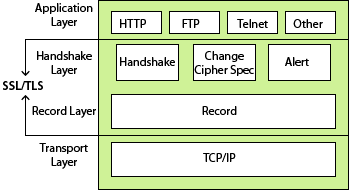
\includegraphics[width=8cm]{SSL-01.png}
\caption{SSL/TLS Protocol Layers}
\label{SSL}
\end{figure}

\subsection{Differences between SSL and TLS}
We find it useful to point out some differences in these two versions of the protocol. Even though they are in general the same, there are some differences.
TLS is based on SSL 3.0, but a machine that is "speaking" TLS would have to run a compatibility protocol connection with a machine "speaking" SSL.
This is mainly due to a difference in the handshaking protocol. During handshake TLS 1.0 will label itself version 3.1. And 3.2 or 3.3 for the respective TLS versions. More importantly is that the verification of the certificate is a part of the handshake for TLS, instead of a separate complex part as in SSL.

Another difference is that TLS is able to switch between secure and unsecured communication on the same port. SSL requires different ports for the two.

TLS has also removed support for FORTEZZA since it is no longer considered secure. One might argue that it should be supported to be able to connect to clients running older versions of SSL. On the other side, security protocols should be kept up to date to fulfill its purpose. Thus supporting old cipher suites will only be a weakness if someone should discover a working cipher suite rollback attack. TLS also allows new cipher suites to be added in the future.

TLS is a bit more careful when creating the cryptographic numbers for RSA  and Diffie-Hellman. Transport Layer Security uses a hashed message authentication code (HMAC) and its pseudo random function (PSF) to generate nonces and such.

\subsection{Encryption}
When a SSL connection is going to be established, the client and the server agrees on four major attributes that is going to be a part of the \texttt{cipher\_suite}. The attributes are a key exchange algorithm, a authentication algorithm, a encryption algorithm and a MAC algorithm. This attributes are finally set in \textit{server hello}. There are several algorithms to choose from in these different attributes. Examples on these algorithms can be:
\begin{itemize}
\item{\textbf{Key exchange}: RSA, Diffie-Hellman}
\item{\textbf{Authentication}: RSA, Diffie-Hellman}
\item{\textbf{Encryption}: DES}
\item{\textbf{MAC}: MD5, SHA, SHA-1}
\end{itemize}

\subsubsection{MAC and HMAC}
\paragraph{MAC} The goal of a MAC is protecting data integrity, but also authentication. Message authentication codes consist of two algorithms. One for signing and one for verifying: \texttt{(Sign, Ver)}. There is a shared key \textit{k} that is shared between the signer and the verifier. The sender computes: $s = Sign_{k}(x)$, where \textit{s} is the signature and the \textit{x} the message. It sends $(x, s)$ to the receiver. The receiver accepts the pair $(x, s)$ from the sender as valid only if $Ver_{k}(x, s) = 1$.

MAC is different from digital signatures since MAC use the same secret key for both generation and verification. That means that client and server must agree on the same key before the connection, this is symmetric encryption. However, digital signatures is generated using the private key of a key pair, this is called asymmetric encryption Unlike digital signatures, MAC do not provide non-repudiation, which could be exploited through a man-in-the-middle attack. A brief definition of a man-in-the-middle attack is given in the section about threats.

\paragraph{HMAC} Hashed message authentication codes is a specific construction for calculating a MAC. It combines a hash function with a secret key. It may be used to simultaneously verify both the integrity of the data and authentication of a message. According to RFC 2104 \cite{RFC 2104} may HMAC be mathematically defined as:
$$ HMAC(K, m) = H((K \oplus op) \parallel H((K \oplus ip) \parallel m)) $$
Where $H(\bullet)$ is a cryptographic hash function, $K$ is a secret key, $m$ is the message to be authenticated, $\parallel$ denotes concatenation, $\oplus$ denotes XOR, $op$ denotes outer padding and $ip$ denotes inner padding. 

\subsubsection{MD5} stands for message-digest algorithm 5, and is specified in RFC 1321. MD5 is used for verifying integrity. It makes a 128-bits (16 byte) long key that contains 32 character of the hexadecimal number system. This algorithm is developed by Prof. Ronald Rivest in 1991. MD5 is not recommended though, after a safety breach was discovered in March 2005. It was proven that two identical 128-bit MD5 keys existed. It is almost unthinkable that this will happen, since it is $2^{128}$ possible key combinations. Recommended algorithm is the Secure Hash Algorithm 1 (SHA-1).

\subsubsection{Symmetric Key} Here both parties got a copy of the same symmetric key. This key is used to both encrypting and decrypting a message. When encrypting a large amount of data, this is computationally faster than asymmetric cryptography. Typical algorithm for symmetric key cryptography can be DES.

\subsubsection{Asymmetric Key} Asymmetric key encryption used a key-pair, where one is public and one is kept private. The public key is used for encryption, while the private key is used for decrypting the message. Anyone may obtain the public key, but the private key is held secret by the owner. If the owner encrypts a message with the private key, anyone that obtain the corresponding public key may decrypt the message. This is the foundation of digital signatures. The most common algorithm for this is RSA.

\subsubsection{RSA}
When this is used for server authentication and key exchange, a 48-byte \texttt{pre\_master\_secret} is generated by the \textit{client}. This is encrypted under the server's \textit{public key}. The server uses its \textit{private key} to decrypt the data. Both parties may then convert the \texttt{pre\_master\_secret} to the \texttt{master\_secret}.

\subsubsection{Diffie-Hellman}
The Diffie-Hellman algorithm was published by Whitfield Diffe and Martin Hellman in 1979. This is a method for key exchanging, it allows two parties to establish a shared secret key over an insecure channel. This is considered secure against eavesdroppers.

\section{Layers}
SSL/TLS is divided into two main layers as shown in figure \ref{SSL}. The upper protocol layer, and the record layer. It is considered two layers seeing as the handshake, the change cipher and the alert protocols are also sent through the record layer. For instance is every message in the alert protocol authenticated and encrypted by the record protocol. This is true for the handshake protocol as well. Though when establishing a connection, no ciphers have yet been selected, so they pass through the record layer without being authenticated or encrypted. It is in total four sub-protocols of those two layers: handshake, change cipher spec, alert and record protocol.

\subsection{The Record Layer}
The record protocol is considered its own layer due to its size and importance. This layer uses SSL in a secure way with message integrity ensured. 
It transmit data over the TCP protocol, and to do that, it goes through several steps. 

The first step for transmitting application data is to fragment the data, breaking it up into smaller pieces. Now SSL will put a header on each data fragment, this header includes the MAC. Now some record data have been constructed, and it includes primary data, some padding and the MAC value.

So what this layer does is to take some application data, fragment it, compress it, apply a MAC and encrypt it, and then you have a TCP packet to transmit.


\subsection{Upper Layer}
This contains the handshake protocol, change cipher spec protocol and the alert protocol.

\subsubsection{Handshake Protocol}
Mainly for key exchange. Initializes and synchronizes cryptography at the endpoints.
In the message flow of the handshake protocol, you include both client and sever. They negotiate a shared cipher suite that both parties can accept. They also agree on a hash algorithm, that is the digital signature. The most common hash algorithms is MD5 and SHA. MD5 produces a 128-bit hash value, while SHA-1 produces a 160-bit hash value.
The \textit{handshake flow} works as follows: 

In \textit{Client Hello}, the client sends the version number equal to the highest it supports, e.g. 3 for SSL 3.0 and 3.1 for TLS. And it generates a master secret that is based on a 4-byte number (the client's date and time), plus a 28-byte randomly generated number. It also contains a list of \textit{cipher suites}. An example of an cipher suite is;
\begin{verbatim}
 TLS_RSA_WITH_DES_CBC_SHA
\end{verbatim}
where \texttt{TLS} is the protocol version, \texttt{RSA} is the algorithm that will be used for the key exchange, \texttt{DES\_CBC} is the encryption alorithm and \texttt{SHA} the hash function.\footnote{This cipher suite example is taken from \url{technet.microsoft.com}'s description of SSL and TLS.}


\begin{table}[h!]
\begin{center}
\begin{tabular}{ p{3cm} |  l |  p{3cm}  }
Client & & Server \\
\hline
\cellcolor[gray]{0.8} Client Hello     & $\rightarrow$   &  \\
\hline
     &  &\cellcolor[gray]{0.8} Server Hello\\
     &    &\cellcolor[gray]{0.8} Server Certificate \\
     & $\leftarrow$    &\cellcolor[gray]{0.8} Server Key Exchange \\
     &    &\cellcolor[gray]{0.8} Client Certificate Request \\
     &    &\cellcolor[gray]{0.8} Server Done \\
\hline
\cellcolor[gray]{0.8}Client Certificate    &   & \\
\cellcolor[gray]{0.8}Client Key Exchange    &  $\rightarrow$  & \\
\cellcolor[gray]{0.8}Certificate Verify    &   & \\
\cellcolor[gray]{0.8}Client Finished Message    &   & \\
\hline
     &   $\leftarrow$  &\cellcolor[gray]{0.8} Change Cipher Spec \\
     &    & \cellcolor[gray]{0.8}Server Finished Message \\
\hline
\end{tabular}
\end{center}
\caption{The Handshake Flow}
\label{handshake_flow}
\end{table}

\subsubsection{Change Cipher Spec Protocol}
This is a tiny protocol consisting of one message. When each end point is ready to start using the agreed encryption, this message will be sent. Once both partied have sent and received such a message, all further communications is authenticated and encrypted with the recently agreed cipher specs.

\subsubsection{The Alert Protocol}

\begin{table}[h!]
\begin{center}
\rowcolors{2}{red}{yellow}
\begin{tabular}{| l |  l |  p{3cm} | }
\hline
Code & Level & State \\
\hline
 1  & warning  & connection may be unstable.  \\
\hline
2 & fatal & connection may be compromised. \\
\hline
\end{tabular}
\end{center}
\caption{Alert Level Types}
\label{alert_level}
\end{table}

The alert protocol consist of one message that may contain a number of alerts. The alerts are divided into two levels as seen in table \ref{alert_level}.

All alerts of the fatal level cause the connection to be ended, and marked as non-resumable. Any failed MAC-validation, failed decryption or other cryptographic failure always give a fatal alert. Warning alerts may be handled as chosen by implementation. Invalid certificated, for instance, may ask the user if he or she wants to use it anyway.

Once a fatal alert has been sent, no more data of any sort will be sent on that connection.


\section{The Strengths of SSL}

\subsection{Cipher suite rollback attacks}
A cipher suite is a name given combination of authentication, encryption and MAC algorithms that is used to negotiate secure network connections at TLS and/or SSL.
SSL 3.0's defense against cipher suite rollback attacks is to authenticate the handshake with a \textit{master secret}.

\subsection{Message Authentication}
Message authentication is important, because of the availability on software that specialize on IP spoofing and TCP session hijacking. This protects SSL through using MAC. MAC protects the integrity. Most commonly is MAC constructed of block ciphers like DES.

TLS however supports HMAC. The hash functions that HMAC uses was not originally designed for message authentication.

For more details about this topic, take a look in the previous section about encryption.

\subsection{Record layer confidentiality and authentication}

\subsection{Replay attacks}
A replay attack as a kind of network attack, where the data transmitted is maliciously or delayed. 

SSL protects itself from this kind of attacks by including a sequence number in the MACed data, this sequence number is refreshed for each new key exchange, therefore no obvious vulnerabilities.

\subsection{Rollback}

\section{Threats}
Here we have described some of the possible threats against the SSL protocol. Ranged alphabetically.

\subsection{Certificate}
\subsection{CPU Performance}
This is not an direct threat against the client sending information over the SSL protocol, but it may be useful to mention that public key encryption is a heavy CPU operation for the server. This is because it have to decrypt the \texttt{pre\_master\_secret} during the handshake process. 

Today there is servers with operative systems that keep this in mind.
\subsection{Dropping Change Cipher Suite}

\subsection{Key Exchange Algorithm Rollback}
An attacker that is present during initial client/server hello messages may successfully defeat all encryption by retrieving the pre-master-secret in a man-in-the-middle attack.

This can be done since the field holding the requested key-exchange protocol is not authenticated, only the parameters for creating the key is. What can then be done is to change the field so that the server thinks it will use the Diffie-Hellman protocol. Now the server believe it is using Diffie-Hellman and the client thinks it is using RSA. The server then sends a prime, \textit{p}, a generator, \textit{g}, and $ g^{x} mod p $, where \textit{x} is the server's nonce. These values can not be changed by the attacker due to public key authentication. What happens now is that the client computes the pre-master-secret with \textit{p} as the RSA modulus and \textit{g} as the RSA exponent. What has happened now is that the RSA computed $k^{g} mod p$ with a prime as its modulus which makes it mathematically feasible to find \textit{k}, the pre-master-secret. The attacker is now in possession of the shared secret and may do as he pleases. 

\subsection{Man-in-the-Middle Attack}
I have chosen to include a little note on these kind of attacks, even though it is not relevant for SSL. SSL can authenticate one or both parties using a certification authority. But as mentioned in the previous section about encryption, MAC does not provide non-repudiation, and therefore may MAC be exploited by these kind of attacks.

A man-in-the-middle attack (MITM) may go on like this:
Lets call the clients involved for \textit{A}, \textit{B} and \textit{C}. And imagine that \textit{A} wants to communicate with \textit{B}, and that \textit{C} wants to eavesdrop and deliver a false message to \textit{B}. To describe the events in an easy was, I'll use this table.

\begin{table}[h!]
\begin{center}
\begin{tabular}{| p{7.4cm} |}
\hline
A: "Hello, B! It's A, give me your key." $\rightarrow$ C $\rightarrow$ B.  \\
\hline
A $\rightarrow$ C "Hello, B! It's A, give me your key." $\rightarrow$ B. \\
\hline
B: [B's key] $\rightarrow$ C $\rightarrow$ A. \\
\hline
B $\rightarrow$ C [C's key] $\rightarrow$ A. \\
\hline
A: "Let's meet at x." [encrypted with C's key] $\rightarrow$ C  $\rightarrow$ B. \\
\hline
A  $\rightarrow$ C: "Let's meet at y." [encrypted with B's key]  $\rightarrow$ B.\\
\hline
\end{tabular}
\end{center}
\caption{Man-in-the-Middle Attack}
\label{MITM}
\end{table}

\textit{B} is tricked to believe the message came from \textit{A}.

\subsection{Traffic Analysis}
The goal of traffic analysis is to attempt to figure out parts of the encrypted message by looking at information that is not encrypted. This is done by instigating non-encrypted packet fields and unprotected attributes in the SSL protocol. SSL does not try to stop traffic analysis. 

When a web-browser (client) connects to a web server, the URL is encrypted. Which web-page that is being downloaded by the client is secret information. However, traffic analysis may restore the servers identity, by looking up the IP destination of the packet and the bit-length of the URL, plus the length of the \texttt{html}-data. The attacker may then do an advanced google search for web-sited with that length name which exists on the respective server. The result of the search will then be which web-page was visited by the client. This will happen because the ciphertext is at the same length as the clear text. A  way to counter this is to add a random number of padding bits.

\subsection{Version Rollback Attacks}
A rollback attack is when a message is being manipulated to represent a less secure version of the protocol than it actually is. 
These kind of attacks are not very successful against SSL, because of the \textit{client key exchange} step of the handshake protocol. Here the client sends a message with MAC to the server. One part of this authenticated message is the version of the protocol, the server will verify that this is the same value as sent in the \textit{client hello} message. 

\section{Conclusion}
\newpage{}
\begin{thebibliography}{}

%Internett
  \bibitem{Technet 03}
    Microsoft. 
    \emph{How TLS/SSL Works}
    Last updated: March 28, 2003. 
    \url{http://technet.microsoft.com/en-us/library/cc783349(v=ws.10).aspx}, 
    downloaded: May 10, 2012.

%Tidsskrift
  \bibitem{ShWa 96}
    B. Schneier, D. Wagner. 
    \emph{Analysis of the SSL 3.0 protocol}.
    USENIX Press, 1996.

    \bibitem{RFC 6101}
       A. Freier, P. Karlton, P. Kocher. 
       \emph{The Secure Sockets Layer Protocol Version 3.0}.
       Netscape Communications. IETF. 
       ISSN: 2070-1721. August 2011.

    \bibitem{RFC 2104}
      H. Krawczyk, M. Bellare, R. Canetti.
      \emph{HMAC: Keyed-Hashing for Message Authentication}.
       Network Working Group. IBM. University of California. June 1996
    

\end{thebibliography}

\listoffigures
\listoftables

%\bibliography{test}{}
%\bibliographystyle{alpha}


\end{document}
